\chapter{Writing a configuration file}
\label{chap:writingconfig}

In this chapter, you will learn the basics for writing a configuration file. We focus on the essential elements, i.e. adding models, datasets, wrappers and preprocessors. For additional features, refer to the next chapter.

\section{Adding a dataset}

Datasets are stored in the ``\textit{datasets}'' folder of the toolbox. They are organized in folders corresponding to the different tasks. To get a summary of available tasks and datasets, run the \verb|info_datasets.m| script.

A new dataset can be added to the simulation with the following syntax:

\begin{small}
\begin{verbatim}
add_dataset(id, name, filename);
\end{verbatim}
\end{small}

\noindent where:

\begin{itemize}
\item \verb|id| is a string identifying the dataset in the configuration file,
\item \verb|name| is a name for the dataset, to be displayed in the results,
\item \verb|filename| is the unique alphanumerical string denoting the dataset in the filesystem.
\end{itemize}

\noindent As an example, the call:

\begin{lstlisting}
add_dataset('Y', 'Yacht', 'uci_yacht');
\end{lstlisting}

\noindent adds the dataset ``\textit{uci\_yacht}'' to the simulation with name ``Yacht''.

\subsection{Adding a multilabel dataset}
\label{sec:multilabeldataset}

You may have seen during the simulation that some tasks have no performance measure assigned to them (e.g., multilabel classification tasks). These may be taught as ``\textit{incomplete}'' tasks, i.e., tasks for which no training algorithms are available. Currently, they are handled by transforming them (after loading the datasets) into other, more ``basic'' tasks. In particular:

\begin{itemize}
\item Prediction tasks are transformed into regression tasks by embedding the timeseries into a phase space.
\item Multilabel classification tasks are transfomed into multiple binary classification tasks (the so-called \textit{binary relevance} method).
\end{itemize}

As an example, try to add a multilabel dataset to a simulation:

\begin{lstlisting}
add_dataset('C', 'Cal 500', 'cal500_mood);
\end{lstlisting}

\noindent You can see that, during initialization, the $36$ labels in the dataset are transformed into $36$ different binary classification datasets:

\begin{console}
Extracted 36 different binary classification datasets from original
  dataset Cal 500
\end{console}

\noindent The $36$ tasks have sequential ids given by C-1, C-2, etc. Similarly, try to add a prediction dataset:

\begin{lstlisting}
add_dataset('M', 'Mackey-glass', 'mackeyglass');
\end{lstlisting}

\noindent During initialization, this is transformed into a regression dataset:

\begin{console}
Embedded dataset Mackey-glass, 4993 samples extracted
\end{console}

How to ``complete'' these tasks, and how to design new ones, are topics explored in the last chapter of the manual.

\section{Adding a model}

A model can be added to the simulation with the following syntax:

\begin{lstlisting}
add_model(id, name, pointer, varargin);
\end{lstlisting}

\noindent where:

\begin{itemize}
	\item \verb|id| is a unique string for identifying the algorithm in the simulation,
	\item \verb|name| is the algorithm's name (to be displayed in the results),
	\item \verb|pointer| is a pointer to the algorithm's class,
	\item \verb|varargin| are the additional parameters to be passed to the constructor of the model.
\end{itemize}

\noindent As in the standard convention of Matlab coding, additional parameters are composed as follows:

\begin{itemize}
	\item One or more required parameters,
	\item One or more additional parameters,
	\item One or more name/value pairs. As a general rule, most parameters are in this form.
\end{itemize}

\noindent For example, the following call:

\begin{lstlisting}
add_model('SVM', 'Support Vector Machine', @SupportVectorMachine);
\end{lstlisting}

\noindent adds a default-initialized Support Vector Machine to the simulation. Similarly, the call:

\begin{lstlisting}
add_model('SVM', 'Support Vector Machine', @SupportVectorMachine, 'kernel_type', 'lin');
\end{lstlisting}

\noindent adds a Support Vector Machine with a linear kernel.

A concise HTML report with a list of all implemented models and respective parameters can be found by calling the script \verb|info_models.m|. Additional information on each model can be found by visualizing the help for the respective class.

\subsection{Changing the training algorithm}

Each model has a default training algorithm, that can be changed with the \verb|set_training_algorithm| function. For example, to change the training algorithm of the previously defined Support Vector Machine to LibSVM:

\begin{lstlisting}
set_training_algorithm('SVM', @LibSVM); 
\end{lstlisting}

\noindent Available training algorithms are listed in the \verb|info_models.m| script.

\section{Adding a preprocessor}

A preprocessor applies some specific transformation to a dataset in the initialization phase. A preprocessor can be added with the following syntax:

\begin{lstlisting}
add_preprocessor(id, preprocessor, varargin);
\end{lstlisting}

\noindent Where:

\begin{itemize}
\item \verb|id| is a regular expression that should match with all the datasets ids to which the preprocessor should be applied,
\item \verb|preprocessor| is a pointer to the preprocessor's class,
\item \verb|varargin| are the additional parameters of the preprocessor.
\end{itemize}

\noindent As an example, the call:

\begin{lstlisting}
add_preprocessor('Y', @PrincipalComponentAnalysis, 'varianceToPreserve', 0.95);
\end{lstlisting}

\noindent applies a PCA transformation to the dataset previously defined, retaining only the principal components encompassing at least 95\% of the variance of the original input.

A list of the available preprocessors is obtained by calling the script \verb|info_preprocessors.m|. Additional information on each preprocessor is given by the help of the corresponding class.

\subsection{Preprocessors and Multi-label Tasks}

The fact that the syntax for adding a preprocessor accepts a regular expression is particularly suited for multi-label tasks. Continuing the example of Section \ref{sec:multilabeldataset}, suppose we now want to perform a PCA on all $36$ binary classification tasks. This can be done with a single call:

\begin{lstlisting}
add_preprocessor('C-.', @PrincipalComponentAnalysis, 'varianceToPreserve', 0.95);
\end{lstlisting}

\noindent The regular expression follows the standard MATLAB convention: in particular, the dot refers to ``any character'', allowing to match all three datasets together. More information on the syntax of regular expressions can be found by reading the help of the built-in \verb|regexp| function.

\section{Adding a wrapper}

A wrapper provides additional functionalities to an algorithm (called in this context its \textit{base algorithm}) by encapsulating its behavior and intercepting inputs and outputs to its training and testing functions. Wrappers can be used for fine-tuning model parameters, extracting or selecting features, saving the models resulting from the simulation, etc.

The syntax for adding a wrapper is similar to the syntax for adding an algorithm:

\begin{lstlisting}
add_wrapper(id, wrapper, varargin);
\end{lstlisting}

\noindent Where:

\begin{itemize}
\item \verb|id| is the ID of the algorithm to be encapsulated,
\item \verb|wrapper| is a pointer to the wrapper’s class,
\item \verb|varargin| are the additional parameters for the wrapper.
\end{itemize}

\noindent Consider as an example the following call:
\begin{lstlisting}
add_wrapper('SVM', @Featuresearch_GA);
\end{lstlisting}

\noindent This adds a wrapper to the Multilayer Perceptron defined in the previous section, that runs a genetic algorithm for searching the optimal subset of features. For details on the implemented wrappers and required parameters, the script \verb|info_wrappers.m| generates a concise report. More information on each wrapper is available by visualizing the help for the corresponding class.

It is important to note that wrappers can pile on top of each other:

\begin{lstlisting}
add_wrapper(ID, wrapper1, ...);
add_wrapper(ID, wrapper2, ...);
\end{lstlisting}

In this case, the \textit{wrapper2} is executed by using as a base algorithm the \textit{wrapper1}, which in turn uses as a base class the algorithm identified by ID. As an example, consider the following code:

\begin{lstlisting}
add_wrapper('SVM', @Featuresearch_GA);
add_wrapper('SVM', @SaveConfiguration);
\end{lstlisting}

\noindent In this case, the first wrapper searches for the optimal feature subset using a genetic algorithm, while the second wrapper saves the resulting configuration, as shown in Fig. \ref{fig:wrappersexample}.

\begin{figure}[t]
\centering
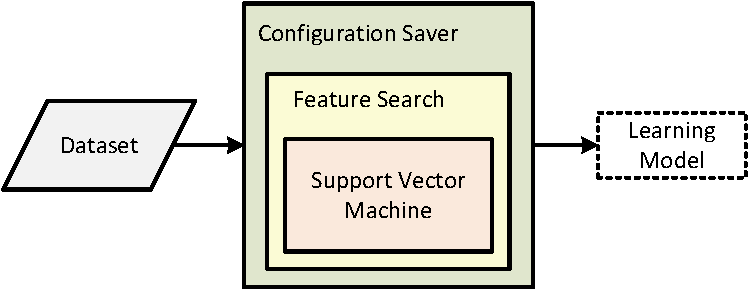
\includegraphics[scale=0.6]{./images/WrappersExample}
\caption{Example of piling two different wrappers}
\label{fig:wrappersexample}
\end{figure}

\noindent The wrappers act at different moments during the learning process: the first one searches the subset before training the final SVM, while the second wrapper saves the configuration after the final training. Other wrappers can have different effects also in the testing phase, allowing for the creation of complex behaviors. For example, an unfolded version of Fig. \ref{fig:wrappersexample} is shown in Fig. \ref{fig:wrappersexample_unfolded}.

\begin{figure}[t]
\centering
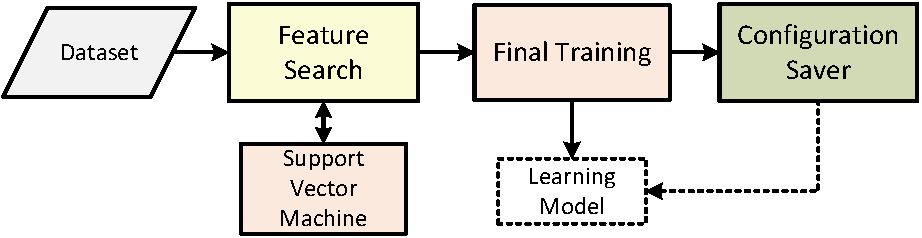
\includegraphics[scale=0.6]{./images/WrappersExampleUnfolded}
\caption{Same as Fig. \ref{fig:wrappersexample}, but with the actions of the wrappers unfolded in time.}
\label{fig:wrappersexample_unfolded}
\end{figure}

\subsection{Example 1: Performing a parameter sweep}
\label{sec:parametersweep}

A very common need in supervised learning is testing a given set of values of one or more parameters of an algorithm, then choosing the combination resulting in the highest level of accuracy. In the toolbox, this functionality is provided natively by the \verb|ParameterSweep| wrapper. As an example of its usage, consider the Extreme Learning Machine (ELM) adopted in the sample configuration, whose simulation has been analyzed in the previous chapter. It has (between others) two tunable parameters, a regularization factor (denoted by \verb|regularizationFactor|) and the number of hidden nodes (denoted by \verb|hiddenNodes|). As is standard practice, we want to test the following range of values for the parameters:

\begin{eqnarray}
2^{-5}, 2^{-4}, \dots, 2^{5} \text{ for the regularization factor}\\
100, \dots, 1000 \text{ for the number of hidden nodes}
\end{eqnarray}

\noindent Since we have two parameters, this results in $10 \times 9 = 90$ configurations to be tested. The following command generates the corresponding wrapper in our example:

\begin{lstlisting}
add_wrapper('ELM', @ParameterSweep, {'regularizationFactor', 'hiddenNodes'}, {2.^-5:5, 100:100:1000});
\end{lstlisting}

\noindent Although this may seem daunting at first, it is actually rather simple. The first parameter is a cell array with the names of the parameters to be tested. The second parameter is a cell array with the values to be tested. By default, this wrapper uses a $3$-fold cross-validation on the training data to test the accuracy. We may change this with any object of class \verb|PartitionStrategy|. For example, to execute an holdout partitioning with $30\%$ of validation data:

\begin{lstlisting}
add_wrapper('ELM', @ParameterSweep, {'regularizationFactor', 'hiddenNodes'}, {2.^-5:5, 100:100:1000}, 'partition_strategy', HoldoutPartition(0.3));
\end{lstlisting}

\subsection{Example 2: saving and loading a configuration}

The second common requirement that we analyze here briefly is that of saving the configuration of an algorithm, for retrieving it in a following simulation. As an example, the grid search of the previous subsection requires training and testing $90$ models, each time performing a $3$-fold cross validation. For large datasets, this requires a very large time, hence we would like to save the results for loading it successively. The \verb|SaveConfiguration| wrapper can be used for saving a configuration:

\begin{lstlisting}
add_wrapper('SVM', @SaveConfiguration, 'ELM_SAVED');
\end{lstlisting}

\noindent After training a model, this will be saved in the ``\textit{./models/}'' folder. Note that a simulation requires training several models, one for each fold, dataset and run. Hence, this will save several files in the folder. The naming convention is that a file is denoted as ID\_DATASET\_rRUNIDfFOLDID.mat, where ID is the id defined above (ELM\_SAVED in our example), DATASET is the name of the dataset, RUNID is the numerical id of the run, and FOLDID is the numerical id of the fold. The saved models can be retrieved on a successive simulation using the \verb|LoadConfiguration| wrapper:

\begin{lstlisting}
add_wrapper('ELM', @LoadConfiguration, 'ELM_SAVED');
\end{lstlisting}